\section{Benchmark NIST-10 "Interior Line Singularity"}
\label{sec:bench-10}

This is another example with anisotropic solution that is suitable for testing
anisotropic element refinements. The equation solved is the Poisson's equation.

\begin{equation} \label{interior}
-\Delta u = f 
\end{equation}

in the domain $\Omega = (-1, 1)^2$, equipped with a zero
Neumann boundary condition on left edge, Dirichlet boundary
conditions given by the exact solution on the rest of the boundary.
The exact solution:

\begin{equation}\label{exact-nist-10}
\left\{
\begin{array}{l}
\displaystyle
u(x,y) = \cos(Ky)\ \ \ \mbox{for}\ x \le 0 \\
u(x,y) = \cos(Ky) + x^{\alpha}\ \ \ \mbox{for}\ x > 0 
\end{array}
\right.
\end{equation}

where $K$ and $\alpha$ are constants.
The right-hand side $f$ is calculated by inserting
(\ref{exact-nist-10}) into (\ref{interior}).
The solution of NIST-10 containing a line singularity with $K = \pi/2$ and
$\alpha = 2.01$ is shown in Fig. \ref{fig:sln-nist10}.

\begin{figure}[!ht]
\centering
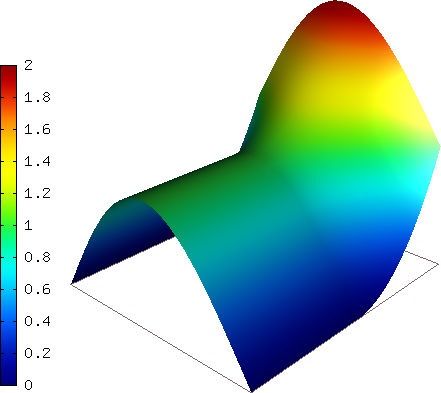
\includegraphics[height=5cm]{nist/nist-10/solution.png}
\caption{The solution to NIST-10 benchmark problem.}
\label{fig:sln-nist10}
\end{figure}

The goal of the benchmark is to reach a relative error below
$10^{-4}$~\% in the $H^1$-norm with as few DOFs as possible.
We begin with adaptive $hp$-FEM,
the initial mesh is shown in Fig. \ref{fig:nist-10-hp-aniso} (left).
After 14 adaptivity steps, the resulting mesh with 381 DOF is shown
in Fig. \ref{fig:nist-10-hp-aniso} (right).

\begin{figure}[!ht]
\centering
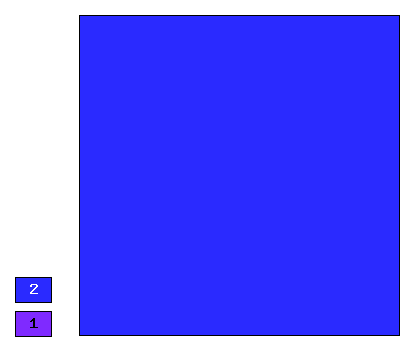
\includegraphics[height=5cm]{nist/nist-10/mesh_hp_aniso_init.png}\ \
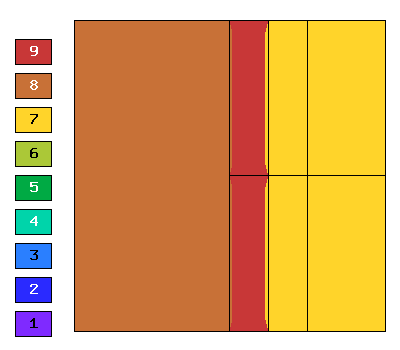
\includegraphics[height=5cm]{nist/nist-10/mesh_hp_aniso.png}
\caption{Initial mesh (left) and final mesh (right) for $hp$-FEM with anisotropic refinements.}
\label{fig:nist-10-hp-aniso}
\end{figure}

The final relative error estimate in $H^1$-norm was 8.68994e-05 \%,
and it was identical to the exact error in all printed digits.
We also solved this benchmark with adaptive $h$-FEM
with linear (left) and quadratic (right)
elements, with anisotropic refinements enabled.
Final meshes for the $h$-FEM computations are shown
in Fig. \ref{fig:nist-10-h-aniso}.

\begin{figure}[!ht]
\centering
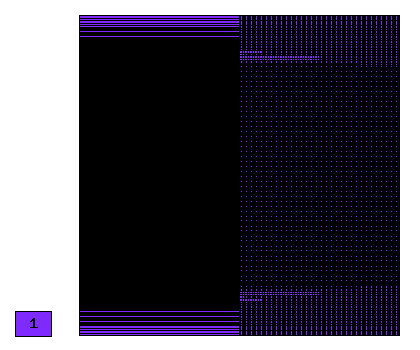
\includegraphics[height=5cm]{nist/nist-10/mesh_h1_aniso.png}\ \
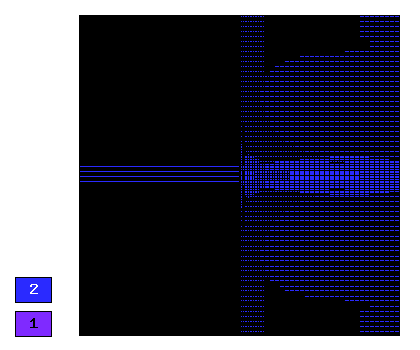
\includegraphics[height=5cm]{nist/nist-10/mesh_h2_aniso.png}
\caption{Final mesh for $h$-FEM anisotropic refinements with linear and quadratic elements.}
\label{fig:nist-10-h-aniso}
\end{figure}

Finally, Figs. \ref{fig:nist-10-conv} compare all
three approaches to automatic adaptivity from the point
of view of DOF and CPU convergence.

\begin{figure}[!ht]
\centering
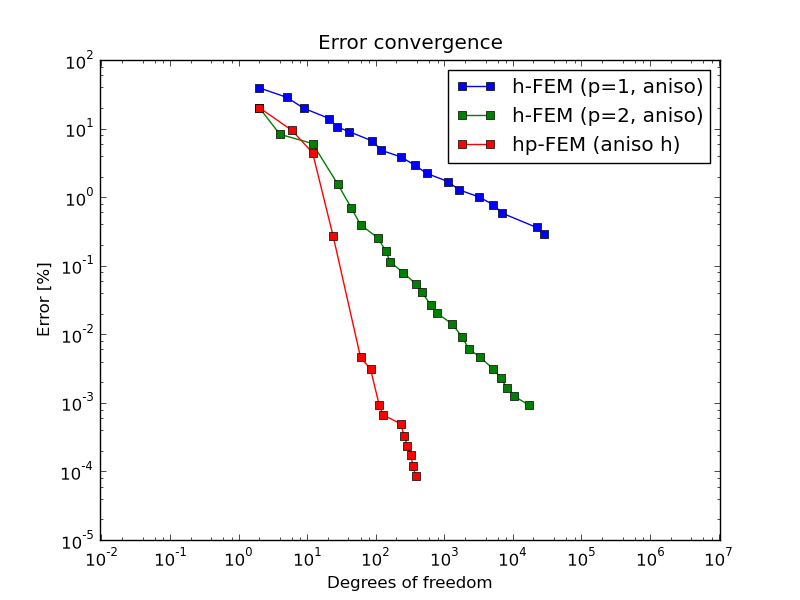
\includegraphics[height=5cm]{nist/nist-10/conv_dof_aniso.png}\ \
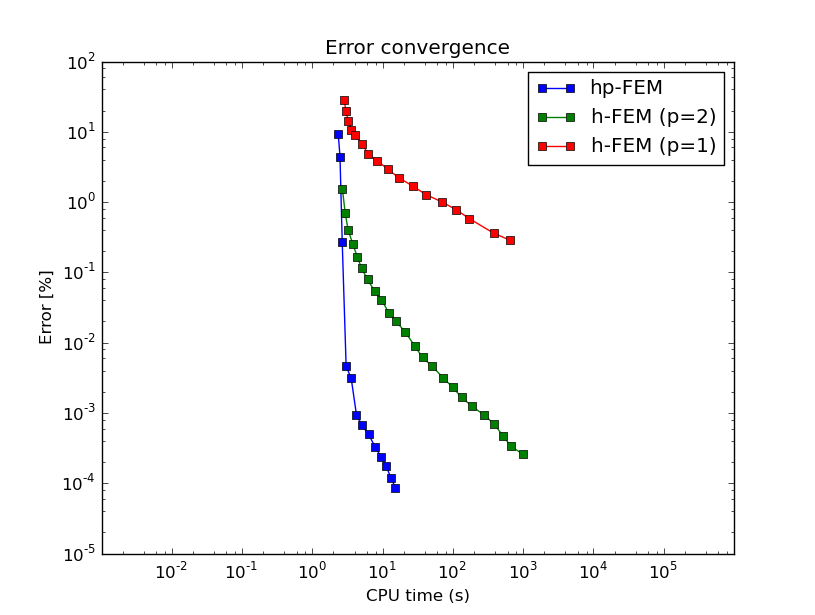
\includegraphics[height=5cm]{nist/nist-10/conv_cpu_aniso.png}
\caption{DOF and CPU time convergence graphs.}
\label{fig:nist-10-conv}
\end{figure}

